\section{Evaluation\label{evaluation}}

Ioa++ permits independent actions to be executed concurrently.
To test this capability, we execute a system whose actions can be configured to span the range from having no independent actions to having all independent actions.
We measure the time required to execute a fixed number of actions using a scheduler with a configurable number of threads.
We then calculate the speed-up by comparing an execution using one thread to an execution using two threads.
We also vary the complexity of each action to gain insight into how synchronization affects concurrent execution.

An automaton $R$ contains an input, output, and internal action.
The output and internal action execute a routine whose complexity is proportional to the parameter $N$.
The automaton executes a fixed number of local actions which was set to 1,000 for all experiments.
The automaton schedules the internal action with probability $\sqrt{\rho}$ and schedules the output action otherwise.
The system $S$ to be executed consists of two $R$ automata composed so the output action of one is composed with the input action of another.
If we divide the execution into rounds where each automaton executes a single action, the probability that both $R$ automata execute an internal action is $\sqrt{\rho} \times \sqrt{\rho} = \rho$.
Thus, we can use the parameter $\rho$ to vary the independence of the automata.

For this experiment, we developed a simple multi-threaded scheduler that assigns each local action to a thread based on the automaton identifier of the local action.
When a single thread is used, all actions are executed by the same thread.
When two threads are used, one thread executes the actions of one $R$ automaton while the other thread executes the actions of the other $R$ automaton.

\begin{figure}
\center
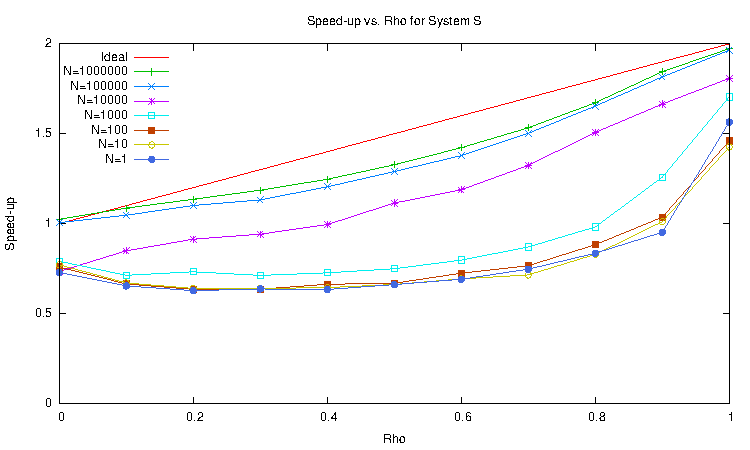
\includegraphics[width=\columnwidth]{speed_up}
\caption{Speed-up for system $S$.\label{speed_up}}
\end{figure}

Figure~\ref{speed_up} shows the speed-up when system $S$ was executed with one and two threads.
The parameter $\rho$ was varied from $0.0$ to $1.0$ in increments of $0.1$.
The parameter $N$ was varied from $1$ to $1000000$ in factors of $10$.
When $\rho = 0$, every action is a bound output action and therefore depends on both $R$ automata.
Consequently, every action must be serialized yielding a maximum speed-up of 1.
When $\rho = 1$, every action is an internal action and can be executed concurrently with a corresponding maximum speed-up of 2.

The speed-up shows a strong dependence on the duration of each local action which is proportional to $N$.
A small value for $N$ means that very little time is spent executing automaton code.
Consequently, a greater fraction of time is spent executing framework code which includes various synchronization calls to the pthreads library.
For a small enough $N$, this overhead dominates the execution time.
This situation is exacerbated by multiple threads since they will actively interfere with one another which can be seen in the slow-down for small values of $N$.
Conversely, when $N$ is large, relatively little time is spent executing framework and synchronization code.
Consequently, contention is reduced allowing for greater speed-ups as indicated by Figure~\ref{speed_up}.

\begin{figure}
\center
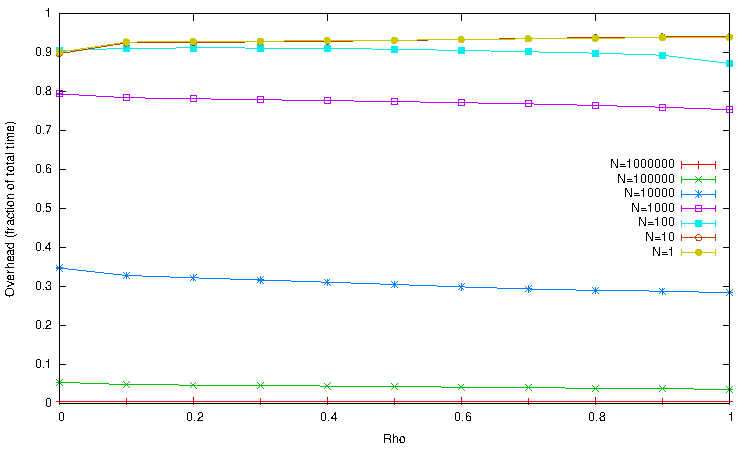
\includegraphics[width=\columnwidth]{overhead1}
\caption{Overhead for system $S$ when using one thread.\label{overhead1}}
\end{figure}

\begin{figure}
\center
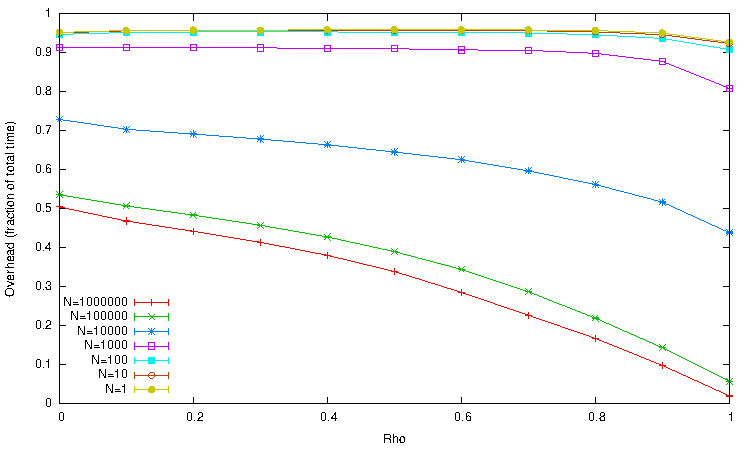
\includegraphics[width=\columnwidth]{overhead2}
\caption{Overhead for system $S$ when using two threads.\label{overhead2}}
\end{figure}

Figures~\ref{overhead1} and \ref{overhead2} show the per thread average of the fraction of time devoted to framework code and synchronization calls for the single and multi-threaded executions.
Since the number of actions to be executed is constant, the single threaded execution shows a relatively consistent fraction for each value of $N$.
The fraction decreases as $\rho$ goes to 1 as the system transitions from acquiring two locks to one lock.
The multi-threaded execution shows that the fraction of time devoted to system overhead decreases as $\rho$ goes to 1 and is more pronounced when $N$ is large.
For example, when $N=1000000$ one thread spends half of its time waiting on the other thread when $\rho = 0$ and spends virtually no time on synchronization when $\rho = 1$.

This experiment indicates that concurrent execution is possible with ioa++ but a speed-up will only be achieved if (1) enough independent actions are enabled and (2) the duration of the independent actions overcome the overhead of ioa++.
The overhead of ioa++ can be divided into three components corresponding to the time it takes to dispatch an action, the time required to synchronize using the pthreads library, and the time required to add an action to the scheduler via the \verb+ioa::schedule+ call.
From the results, we calculated the average overhead per action of the ioa++ framework when dispatching an action and found it to be 4211.5ns with a standard deviation of 765ns for the single threaded experiments and 4858ns with a standard deviation of 1099ns for the multi-threaded experiments.
Similary, we calculated the scheduling overhead and found it to be 227.5ns with a standard deviation of 62ns for the single threaded experiments and 27.9ns with a standard deviation of 79ns for the multi-threaded experiments.
Both of these can be improved with better scheduler design.
The synchronization time depends on the interactions among the system being executed, the scheduler, and the locking scheme used by the framework.
We plan to address scheduling and synchronization in future work.
